\section{Introduction}
Scientific organization is usually treated as the setting in which research
occurs: institutions allocate resources, evaluation selects work, publication
circulates results, and careers affect future participation. These arrangements
can instead be design variables. Given an explicit objective, which organizing
system would an optimization process construct, and what would it make
researchers do differently? This question concerns the system that coordinates
science, not only tuning an acceptance rate or automating an individual scientist.

ScienceUtopia supplies a persistent, literature-grounded LLM-agent ecosystem
with research, submissions, peer review, publication, funding and longitudinal
researcher state~\citep{jin2026scienceutopia}. We extend that world rather than
replace it with a smaller numerical model chosen for convenient gradients.
The original organization is one representable instance, not the upper bound
of the institutional language. Review is an example, not a mandatory family:
new organizing programs may alter information flow, planning, resource
allocation, communication or the relations among mechanisms.

The central separation is between \emph{what can change} and \emph{how it is
searched}. Parameters, algorithms, added mechanisms and rewired processes form
a spectrum of design freedom. Random proposals, loss-feedback program search,
continuous optimization and score-function estimation are methods that can act
on different parts of that spectrum. An institution need not be globally
differentiable to admit useful optimization. Conversely, writing a tensor
representation or computing a derivative is not evidence that the derivative
faithfully predicts the native research world.

\begin{figure}[t]
\centering
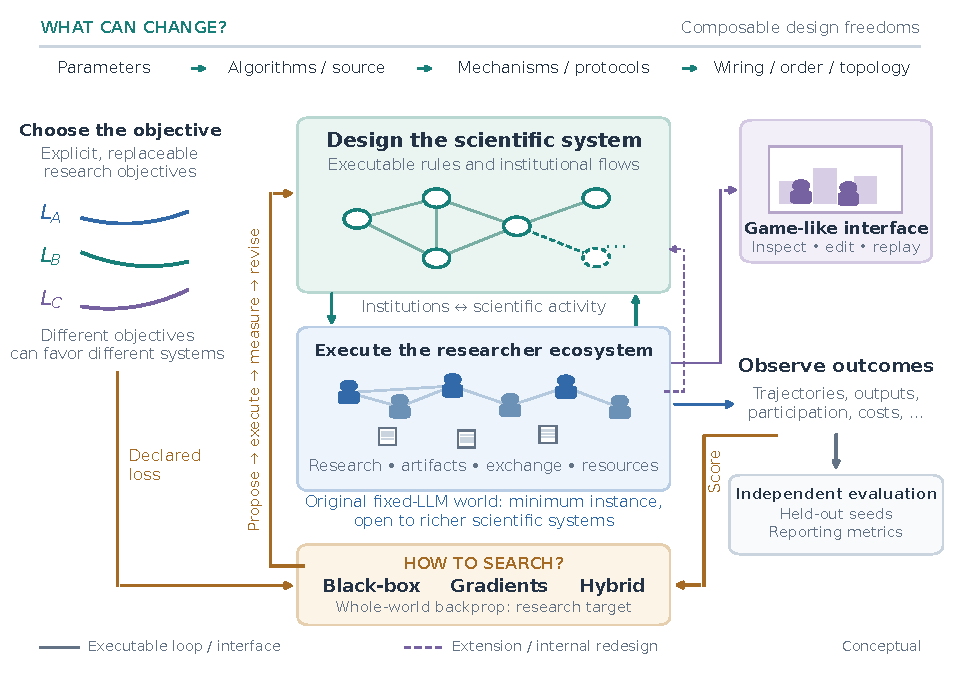
\includegraphics[width=\linewidth]{figures/program-concept/science-system-design-program.pdf}
\caption{\textbf{Research program: optimize scientific organization.}
The objective, the editable system and the search method are separate objects.
Parameters, algorithms, mechanisms and wiring/processes are design freedoms,
not four optimizer names. The native world is contained rather than replaced.
The diagram describes the research space, not proof that every experiment
uses every freedom or that any method improves scientific truth.}
\label{fig:integrated-concept}
\end{figure}

\paragraph{The research contribution and its scope.}
We present an executable formulation of scientific-system design, an integrated
native execution/search/evidence interface, and a sequence of bounded studies
that test different parts of the formulation. Parameter search demonstrates
objective-dependent selection and uncertain held-out profiles. External-author
cases establish that new source, protocols, project processes and feedback
routes can execute in the original world. Gradient studies distinguish exact
local computation, approximate response representations and conditional
expected-loss gradients. A matched local-designer study tests permitted
freedoms against stronger references without dropping failures. The game-like
interface makes the same designs and observations inspectable.

Code-defined agent search, mechanism synthesis and scientific harness
adaptation are existing research directions, not claims of priority made here
\citep{narayanaswami2022programmatic,hu2024adas,wu2026scimars}.
Our empirical target is the map from a declared objective to an executable
organizing system, its native behavioral consequences and its unused-condition
profile. Identifying that object does not yet establish a general result about
the value of free institutional design; the bounded studies below retain that
gap rather than claiming novelty for a generic propose--evaluate--revise loop.

These are not claims of a new optimization identity, a universally good
scientific institution or a trained self-improving inventor. The main empirical
tension is that \emph{representational freedom, exercised institutional change
and effective optimization are different achievements}. Wider permission
does not guarantee a submitted program; a new node need not improve loss;
a lower proxy need not improve science. The experiments make these differences
observable rather than enforce a favorable outcome.

\subsection*{Evidence at a glance: what supports which claim?}
\label{sec:evidence-at-a-glance}
The central empirical question is not whether an institution can be encoded,
or whether a chosen proxy can be made smaller than a weak starting system.
It is whether objective-conditioned search finds consequential organizing
rules beyond strong same-authority alternatives, and how those rules act in
the persistent researcher world. Table~\ref{tab:claim-evidence-map} separates
the strongest completed comparisons from claims they do not establish.
The table is a reading map, not a pooled estimate or a declaration that the
research program is publication-ready.

\begin{table}[t]
\centering\small
\setlength{\tabcolsep}{3pt}
\begin{tabular}{@{}>{\raggedright\arraybackslash}p{.20\linewidth}>{\raggedright\arraybackslash}p{.41\linewidth}>{\raggedright\arraybackslash}p{.33\linewidth}@{}}
\toprule
Completed comparison & Supported observation & Not established \\
\midrule
Matched local search (Section~\ref{sec:matched}) &
120 slots: 64 complete, 25 generation nulls, 31 execution nulls. After frozen
selection, 90 physical evaluations of 15 exact policies retain stronger rules:
throughput code, technical-only and uniform selections average 6.2 acceptances,
tying all-accept; LLM numeric retains the seed at 0.2. Review-cost code selections
average loss 1.92, worse than reviewer-free reject at 0. &
Free-design or feedback superiority; structural invention. The 90 jobs are
not 90 independent optimization histories. \\
\addlinespace
Same-authority topic rules (Section~\ref{sec:native-topic-system-search}) &
Two hand-written rules yield 20 versus 36 accepted decisions at equal
collected cost 200. Original topic durations and scientist weights are fixed;
actual topics and subsequent researcher inputs differ. &
Automatic discovery, duration-only mediation or a world-level optimum. \\
\addlinespace
Terminal resource rule (Section~\ref{sec:native-terminal-cost}) &
A hand rule improves declared resource-aware loss by 4: collected cost
200$\to$160, unpaid cost 0$\to$40, requested cost still 200. All 179 scientist
inputs/literal choices and 36 accepted records match. &
Less requested work, better science, an invented institution or long-run benefit.
The gain is retained, not disqualified. \\
\addlinespace
Source-information search (Section~\ref{sec:native-consumer-source}) &
Eight own slots retain seven completed outcomes and one native null. All four
frozen own selections tie the strong visible rule; an adverse path recovers a
supplied rule rather than a new best-known program. &
A general negative effect of source access, an impossibility of useful
institution search or a clean isolated measure of understanding. \\
\bottomrule
\end{tabular}
\caption{Evidence and inference boundaries. Losses and budgets belong to their
own studies; matching symbols do not make them a common benchmark. Hand
controls establish reachable effects but are not discoveries by the local
inventor. Technical nulls remain unavailable measurements, not bad numeric
scores. Complete programs, all attempts, costs and separate conditions remain
in the corresponding sections and appendices.}
\label{tab:claim-evidence-map}
\end{table}

\paragraph{Loss symbols are study-local, not interchangeable metrics.}
In the matched V2 study, $T=-A$ and $C=4A-Q+0.1R$: $A$ counts accepted
decisions, $Q$ sums their native peer scores and $R$ counts reviews. In the
later content/resource studies, $L_U=-U$ and $L_C=-U+0.1K$: $U$ sums centered
opinions from a fixed external abstract-content observer, while $K$ is
collected native activity cost. Native peer scores and external opinions are
different measurements; review counts and collected resource units are
different costs. Neither objective is retrospectively substituted for the
other. The historical parameter objectives and their unused-condition
evaluation remain separately defined in Section~\ref{sec:parameter}.

\paragraph{A completed finite search is not a method advantage.}
At November 16, 2026, 14:05 UTC, the later priority/free-method writer exits
normally with all 24 own observations and three references. Twelve own
observations tie and 12 worsen their visible reference; none improves it.
The 12 frozen own-only selections yield eight ties and four worse losses.
The full original paired cold/cost/readout chain is still running at the
14:11 UTC verification. Section~\ref{sec:native-priority-method-snapshot}
includes all 24 slots, while older dated receipts remain unchanged. Its author visibility/phase
defect prevents isolated attribution to objective or method; prospectively
corrected software is not an observed corrected search result. Literal
24-slot values, frozen selections and original input bindings are retained in
\path{research/results/native-priority-method-terminal-snapshot-v1.json}.

The earlier structural, gradient, nested-design and English game-interface
tracks also remain in this manuscript. Their different authors, sources and
conditions cannot be added to the matched local experiment as independent
replications. Available design freedoms and available optimizers are not
themselves evidence that those freedoms are useful or that any optimizer
improves expected institutional performance. A focused main-track claim and
adequate independent evidence remain open, even though substantial software
and finite studies are complete.

\section{Problem: objectives select organizing systems}
\label{sec:problem}
Let $S\in\Sys $ specify an organizing system, $W$ researcher-model weights, $D$
the literature corpus, $ c $ an environmental condition and $\epsilon $ residual
execution/model randomness. The native simulator generates a trajectory
\begin{equation}
 \tau\sim P(\cdot\mid S,W,D,c),\qquad m=M(\tau).
\end{equation}
It contains research directions, projects, papers, review and publication
records, resources, messages and persistent state. A declared loss $\ell_\lambda $
defines the design problem
\begin{equation}
 J_\lambda(S)=\mathbb E_{c,\epsilon}[\ell_\lambda(M(\tau))],\qquad
 \text{seek }S\text{ with small }J_\lambda(S).
 \label{eq:integrated-objective}
\end{equation}
Finite observations estimate only their declared conditions. A single saved
trajectory is neither an exact expectation nor a global optimum. Weights $W$
are fixed within each experiment, but behavior is not: a different information
route, resource state or publication history changes future LLM inputs.

\subsection{Loss, validity, evaluation and adoption}
Four contracts have different jobs (Table~\ref{tab:integrated-contracts}). The
optimized loss selects candidates. Technical validity checks whether an
observation can be obtained under the declared execution and budget contract.
Outside metrics and unused conditions characterize selected systems.
An optional adoption policy governs deployment, not the search objective.

\begin{table}[t]\centering\small
\caption{Four separate contracts. No substantive veto is implicit.}
\label{tab:integrated-contracts}
\begin{tabular}{@{}>{\raggedright\arraybackslash}p{.19\linewidth}>{\raggedright\arraybackslash}p{.49\linewidth}>{\raggedright\arraybackslash}p{.22\linewidth}@{}}
\toprule
Object & Question answered & Search role \\
\midrule
LossSpec & Which measured system is preferred under this objective? & Proposal feedback and selection \\
Validity & Did literal code execute and yield the required measurements? & Numeric loss or explicit null \\
Evaluation & What happens under other scores or unused conditions? & Withheld when declared held out \\
Adoption policy & Should a measured institution be deployed? & Separate, only if explicitly chosen \\
\bottomrule
\end{tabular}\end{table}

An execution failure has a missing loss, not an invented large penalty or a
zero score. We retain the consumed slot, draft, error and observed cost. An
objective may select a normatively unattractive institution: we do not reject
it through an undeclared fairness, novelty, participation or improvement floor.
This does not mean technical completion makes the institution desirable.
If evaluation informs the next proposal, it is development feedback rather
than held-out evidence.

\subsection{Objective design is a scientific question}
Science-of-science research motivates examining careers, knowledge production,
collaboration, diversity and institutions jointly~\citep{fortunato2018science}.
Responsible research assessment also cautions against equating a metric with
the mission it is meant to assess~\citep{hicks2015leiden}. We use this perspective
to expose objective choices, not to declare one official national-policy index
the universal target. Publication counts, topic entropy, review scores,
participation and resources can each be optimized or diagnosed; their role
must be declared before a campaign.

Optimization creates a further distinction: a useful measurement for describing
a fixed system may become a poor objective once the system can change its
measurement-generating process. A program can reduce review work by omitting
review, raise throughput by changing project timing, or select historically
favorable reviewers. Those are possible answers to a declared proxy, not
automatic evidence of epistemic progress. We therefore preserve raw components
and cross-objective profiles instead of reporting only a winner's scalar.

\section{An executable space of scientific systems}
\label{sec:design}
\subsection{Specifications, implementations and composition}
A \Spec{} declares actor/artifact types, mechanism instances, input/output ports,
directed connections, temporal latency, schedules, initial state and invariants.
A mechanism specifies an implementation and its parameters/state contract. Its
implementation can be native trusted code, isolated authored Python, an LLM
operation or a supported tensor representation. A fingerprint covers literal
specification bytes after canonical serialization; it is identity evidence,
not a measure of algorithmic novelty.

The design freedoms are related but should not be collapsed into a fixed menu:
\begin{enumerate}[leftmargin=*,nosep]
 \item \textbf{Parameters}: change settings within a fixed implementation and graph.
 \item \textbf{Algorithms}: replace executable mappings or state updates behind
 a compatible interface, not merely select a named policy.
 \item \textbf{Mechanisms}: introduce or remove actors, storage, decision services
 or source-defined institutional components with explicit consumers.
 \item \textbf{Wiring and processes}: change who receives what, when it arrives,
 the dependency order, conditional invocation and bounded repetition.
\end{enumerate}
Study-specific domains can restrict these freedoms for comparison. A valid
schema does not make every imaginable graph executable in a particular world.
For example, an empty graph may be structurally well formed but fail the
native observation contract. Omitting review requires a compatible downstream
decision consumer; the host does not invent missing reviews or silently repair
the publication rule.

Graph syntax and operational authority are different. An arbitrary program
with the same observations, state and invocation opportunities may implement
several mechanisms inside one policy. Conversely, a program invoked only
after review cannot undo the reviews already performed in that period.
Comparisons must therefore specify available observations, effects and
execution times, not only node count or the label ``free graph.'' A restricted
parameter family can lack an operation even when another code representation
could express it. Section~\ref{sec:design-diagnostics} examines these boundaries
without claiming that graph syntax is universally necessary.

\subsection{Containment of the original researcher world}
\code{NativeScienceKernel} executes specifications against the original
Simulation lifecycle. Default nodes delegate to its phase methods rather than
approximate scientist behavior numerically. A private annual frame retains
native domain objects; versioned JSON ports expose bounded records to authored
mechanisms. Review selection is separable from publication commit, so new
decision code can still affect the actual paper tracker, retrieval archive,
resource state and later researcher prompts.

Default behavior has deterministic native-lifecycle checks comparing scientific
state, RNG state and full request payloads under matching scripted replies.
These are engineering containment tests, not new Qwen experiments. The live
studies below separately use fixed local Qwen3-8B scientists and actual
literature-grounded native forwards. They are small local settings, not a
reproduction of the source paper's reported Qwen3-32B configuration.
The local four-year literature subset contains 103,107 CS records from 2016--2019,
drawn from SciEvo~\citep{jin2024scievo}. Corpus and retrieval identities are
bound separately from the researcher model; a local run is not a replication
of the source paper's model scale or full experimental population.

The extension is conservative, not unlimited. Generated code cannot import
arbitrary host objects, change researcher weights, rewrite a measurement or
invent a trusted capability by naming it. Annual native phase handlers retain
their own scientific semantics. A new kind of real activity needs an implemented
consumer, identity/accounting transport and measurement interpretation; a
record called ``discovery'' does not become a validated discovery.

\paragraph{Native effects versus a fixed historical calendar.}
The later workflow domain fixes native effect contracts rather than their
annual schedule. It permits institutional code, nodes and typed wiring while
requiring exactly-once protected effects, producers before zero-latency
consumers, opening before activity and ledger closure after mutations.
Descriptive ordering metadata is not execution authority. A structural-only
experiment can then hold sources, parameters and nodes literal and change
phases/connections alone; that experimental restriction is not the general
system language's ceiling. A hand timing control changes three phases and
five edges without rewriting any native effect. Its fresh scientist-world
loss is an empirical question, not a consequence of graph validity.
The complete new-binding software check uses seven SCRIPTED native worlds,
28 annual checkpoints, 13 bounded mock-HTTP workers and a retained generation
null, with matching double audits, costs and reports. This exercises original
production and cold readers, not real-model workflow invention or improvement.

\subsection{New institutions and their actual consumers}
Isolated Python receives declared inputs and state and returns schema-checked
outputs/state. It can implement an entirely new algorithm, generate intermediate
protocols or maintain institutional memory. It runs in a pinned, network-disabled
container, not as model-supplied code imported by the host. Output shape,
identities and required port coverage are checked; scientific merit is not.

The domain bridge supplies generic effects: persistent actor/artifact creation
and revision, namespaced state, delivery of arbitrary linked records to real
researchers, actual project-plan changes and conserving resource transfers.
Roles and schema-declared state are data; source supplies the institution's
allocation or communication rule. New actor serialization alone does not
provide autonomous behavior. Custom artifacts can link native papers but do
not increase accepted-paper counts merely by being stored.

Information must reach a consumer to matter. A message route records producer,
port, event lineage and recipient. Researcher context delivery modifies actual
LLM requests; decision outputs address real submitted papers; plan amendments
alter actual native project state. Execution receipts can establish delivery
and committed effects. Neither a node label nor the designer's explanation
establishes that the changed code ran, was read or caused a better outcome.

\subsection{Processes, time and state}
Dependencies and typed data edges define deterministic within-period ordering.
Delayed edges carry records to later periods. Controlled activities support
source-authored Boolean guards, bounded counts, persistent state and explicit
termination. Missing control can be declared a wait or an error; a skipped
activity is not fabricated research. Bounds are execution budgets, not merit
filters. Original single-shot annual handlers cannot simply be repeated with
their old IDs and side effects. Richer repetition requires repeatable activities
with genuine invocation identities and domain effects.

Checkpoints retain mechanism state, queued messages, actors, artifacts and
source binding. Resume cannot silently switch to a different institution.
This supports longitudinal feedback within a world. Most reported optimization
trials, however, reset their worlds: repeated candidate evaluation is not the
same as one society recursively redesigning itself over time.

\section{Search methods and gradient boundaries}
\label{sec:search}
\subsection{A common propose--execute--measure loop}
The persistent controller accepts a loss, initial specification, design domain,
information policy and finite budget. It saves a proposal before dispatch,
validates its literal transaction, executes a native forward, measures canonical
loss and updates eligible search history. The generic ask/tell boundary does
not require simulator derivatives. A domain adapter, not the optimizer,
understands coordinates, source replacements or graph transactions.

Black-box optimization includes uniform sampling, incumbent mutation,
local refinement and LLM proposals. The implementation supports an objective
and own-history archive, not an obligation to change or improve a candidate.
Repeated designs, worse revisions and ties consume their scheduled budget.
The host does not rewrite generated code, manufacture a terminal submission
or replace a failed slot. Trace-informed designers may inspect more than a
scalar oracle; such comparisons must disclose their richer information.

An LLM designer can emit executable definitions and structured patches. The
execution engine checks the resulting program rather than interpreting prose
as functionality. In the local matched study, the scientist and designer are
different fixed models. External-author pilots have different provenance:
they establish expressive examples and observed redesign, not local-model
invention or an authenticated independent designer identity.

\subsection{Pathwise derivatives of explicit representations}
For a supported differentiable institution $ u=f_\theta(x)$, a local backward
pass computes derivatives of that represented mapping. Tensor state and
explicit routes can carry derivatives through multiple represented operations
and invocations. Such a derivative is exact for that computation, not for an
opaque LLM, retrieval, integer parser or unrepresented native transition.

A conditional response operator $\widehat r_\phi(x,\theta)$ fitted to native
observations can supply missing response sensitivities in an approximate
path. Autograd then computes $\nabla_\theta\widehat L$, not automatically
$\nabla_\theta J$ of Eq.~\eqref{eq:integrated-objective}. Hard selection may be
relaxed by smooth probabilities while the native forward remains hard.
Temperature changes both fit and sensitivity. A low calibration error does
not establish accurate unused-condition predictions, and a useful local fit
does not make arbitrary generated source differentiable.

We keep represented derivatives, native perturbations and projected native
reevaluations separate. Opaque links remain unknown, not zero-imputed. If a
hybrid proposal combines estimates from several sources, its target, bias
and eligible data must be named; blending estimates is not an unbiasedness proof.
The native-response experiments in Section~\ref{sec:gradient-evidence} examine
this boundary directly.

\subsection{Expected-loss gradients around an opaque world}
Let a fixed generated vocabulary $V$ map explicit discrete choices and continuous
latents $ d $ to $S(V,d)$. For a declared distribution $ q_\theta(d\mid V)$,
\begin{equation}
 J_V(\theta)=\mathbb E_{d\sim q_\theta,\,\tau\sim P(\cdot\mid S(V,d))}
 [\ell(M(\tau))].
\end{equation}
Under support, integrability and differentiation conditions, and with no
additional direct $\theta $ dependence of the conditional environment,
\begin{equation}
 \nabla_\theta J_V
 =\mathbb E[(\ell-b)\nabla_\theta\log q_\theta(d\mid V)].
 \label{eq:integrated-score}
\end{equation}
This standard likelihood-ratio identity estimates a design-distribution
gradient without a world Jacobian~\citep{parmas2021unified}. It covers the
explicit categorical/Gaussian design law, not unknown probabilities of arbitrary
LLM source synthesis or researcher text. Fixed transforms from unbounded
latents to legal coordinates make the sampled density and executable value
distinct objects that must both be retained.

For $K$ IID design draws, leave-one-out baselines exclude the scored draw's
own loss. For a prior-frozen surrogate $ c(d)$ with tractable expectation,
\begin{equation}
 \nabla_\theta J_V
 =\mathbb E[(\ell-c(d))\nabla_\theta\log q_\theta(d\mid V)]
  +\nabla_\theta\mathbb E_{q_\theta}[c(d)].
 \label{eq:integrated-control}
\end{equation}
The correction matters; inaccurate controls need not bias this identity but
can increase variance. Fitting on the current scored batch or omitting the
correction changes its justification. Composable gradient frameworks and
composite estimators motivate these interfaces, not a claim to have reproduced
their complete algorithms~\citep{parmas2022proppo,parmas2023composite}.

Validity-dependent missing losses need special care: discarding failed draws
does not automatically estimate the unconditional expectation above. We keep
null batches and unavailable updates explicit. A campaign may instead declare
a failure-valued estimand in advance, but these studies do not invent one after
observing failures. A computed update and a distribution actually evaluated
after that update are also separate evidence.

\subsection{Changing the design language itself}
An outer author can use its own measured history to change $V$: new source,
mechanisms, factors, coordinate meanings and wiring. Inner score updates stay
conditional on the current $V$. If an outer revision removes a coordinate or
changes its meaning, old gradients/control state are not silently transported.
A point-mass design or retaining the incumbent is legal. Section~\ref{sec:nested}
executes this outer-design/inner-update composition in the original world.
It is an application of existing search and estimation ideas, not a new
theory of differentiable program synthesis.

\subsection{What finite searches and fixed-policy comparisons estimate}
\label{sec:finite-estimands}
Let $\mathcal C_{\lambda mh}$ be the declared eligible candidate pool for
objective $\lambda$, proposal method $m$ and design history $h$. Eligibility
here means the protocol's selection pool, not a hidden scientific-merit test.
Write $\mathcal V_{\lambda mh}\subseteq\mathcal C_{\lambda mh}$ for the
complete eligible designs. After development, retain the entire observed minimum set
\begin{equation}
 \mathcal B_{\lambda mh}=
 \mathop{\mathrm{arg\,min}}_{S\in\mathcal V_{\lambda mh}}
 \widehat L^{\mathrm{dev}}_\lambda(S),
 \label{eq:finite-minimum-set}
\end{equation}
and apply only the predeclared tie rule to choose an evaluation specification
$S^*_{\lambda mh}$. Equal losses do not establish equivalent programs or
identical trajectories. An initial/reference policy belongs to the pool only
when that protocol makes it eligible; submitting an unchanged reference is
legal but is not new invention. An empty eligible complete pool leaves an
unavailable selection, not an automatically substituted baseline.

For a fixed selected policy and an explicit reference $S_0$, the common-condition
comparison is
\begin{equation}
 \Delta_{\lambda mh}(c)=
 L_\lambda(S^*_{\lambda mh};c)-L_\lambda(S_0;c).
 \label{eq:reference-relative-loss}
\end{equation}
Negative values favor the selected policy under that same objective. Different
losses need not have comparable units, so comparing the magnitudes of T and U
is not a method ranking. A common world seed names a matched environmental
condition, not identical residual LLM randomness after two policies generate
different requests. Pairing is therefore by declared condition and actual
observations, not by an assumption that every stochastic event is shared.

Variation over unused $c$ characterizes the already selected policy. Variation
over independently repeated $h$ is also needed for an expected claim about the
search procedure that selects it. More evaluation seeds for one selected
specification do not become more independent optimization histories. Pooling
several development histories into one winner likewise yields one selected
policy per arm, not one held-out result per history. Different source snapshots,
design domains, horizons and observers below are not pooled into a method
effect.

A technical null in either member makes that pair's loss difference unavailable.
All attempted, failed and unattempted slots remain visible with their actual
costs. Reporting loss only for completed pairs is conditional evidence and
must accompany coverage; it is not an unconditional end-to-end risk estimate.
No retrospective failure penalty is introduced to obtain a numerical ranking.
Cross-objective scores reuse a trajectory's measurements when available;
they are not additional world samples. Cached judgments of identical content
similarly remain the same physical opinions, not independent replications.

The objective-to-system question includes both its selected outcomes and its
path: literal revisions, exercised effects, native consequences and cost.
Different objectives may return overlapping minimum sets. If the objective
also changes a loss-selected editing parent, the contrast concerns the entire
objective-conditioned search, not scalar feedback alone with the parent held
fixed. None of these definitions requires different winners or a positive gain.
\FloatBarrier
